\input{sep3-annotated-ott}
\input{sep3-unannotated-ott}

\renewcommand{\Sepdrulename}[1]{\scriptsize \textsc{#1}}
\renewcommand{\SepUdrulename}[1]{\scriptsize \textsc{#1}}
% See the seppp.tex file for reminders of the motivation of the
% design.

The previous chapter introduced the freedom of speech
dependently-typed functional programming language. This language
contained two fragments, the logical fragment and the programmatic
fragment.  However, these fragments are judgmentally kept separate.
That is the syntax was the same for both fragments, even more so the
syntax for programs and types are collapsed into a single syntactic
category.  Thus, the fragments are not strictly separate, but rather,
weakly so.  This particular design is very appealing because it has an
elegant definition, but this elegance comes at a cost.  The type
system suffers from many value restrictions, and as we have said
above, this makes programming very hard.

Consider a design where instead of a weak separation of the two
fragments -- logical and programmatic -- we insist on a strict one.
That is the logical fragment and the programmatic fragment have
completely distinct languages for types and programs, and then the two
fragments are related using freedom of speech by typing rules.  So we
go from a picture that looks like this:
\begin{center}
  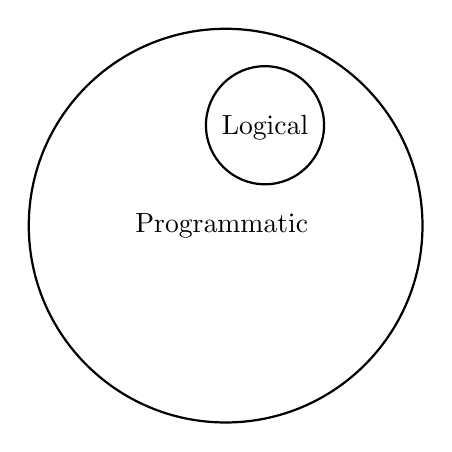
\begin{tikzpicture}[scale=2.5,cap=round,>=latex]    
    \draw[thick] (2.8cm,0cm) circle(1cm);
    \draw (2.78cm,0cm) node {Programmatic};
    \draw[thick] (3cm,0.51cm) circle(0.3cm);
    \draw (3cm,0.5cm) node {Logical};
  \end{tikzpicture}
\end{center}
To the following picture:
\begin{center}
  \begin{tikzpicture}[>=stealth',shorten >=1pt,auto,node distance=5 cm, scale = 1, transform shape]
    \node[state, minimum size=83.1pt] (A)              {Logical};
    \node[state] (B) [right of=A] {Programmatic};

    \path[->] (A) edge [bend left] (B)
              (B) edge [bend left] (A);
  \end{tikzpicture}    
\end{center}
We have seen this diagram before in the previous chapter, but there it
was used to give an intuitive understanding of the free speech
property, but the two fragments are not strictly separate.  Now we
insist that they are in fact strictly separate, and the first diagram
above is no longer applicable; unlike the freedom of speech language.  We
will see that this separation allows for the lifting of all value
restrictions from the typing rules.  

The freedom of speech language is not a very expressive programming
language.  For example, we did not show how to construct full
programs, nor did freedom of speech contain any notion of abstract
data types or pattern matching.  Thus, it is rather difficult to
consider freedom of speech as a real-world programming language.  In
this chapter we introduce the design of a new programming language
called Separation of Proof from Program ($\Sep$) that contains all of
these new features.  The logical and programmatic fragments are
strictly separate, and $\Sep$ is a full real-world programming
language complete with abstract datatypes and pattern matching.  There
are also additional features that we will introduce below.  The
definition of $\Sep$ is very large with over a hundred typing rules
and a large amount of syntax.  Therefore, we do not have the space to
introduce the complete definition in the same style as we did for
freedom of speech, but instead concentrate on the most important
aspects of the design.  If the reader wishes to wade through the
entire definition, then please see
Appendix~\ref{sec:annotated_separation_of_proof_from_program} and
Appendix~\ref{sec:unannotated_separation_of_proof_from_program}, but
the reader may wish to read this chapter first to understand the need
for two appendices.

$\Sep$ consists of two distinct phases: compile time and runtime, and
$\Sep$ separates each phase into its own language.  The compile time
phase uses the annotated $\Sep$ language, and the runtime phases uses
the unannotated $\Sep$ language.  The former is then translated into
the second using an meta-level function called the eraser.  This
function removes the annotations from objects of the annotated
language yielding objects of the unannotated language, furthermore, the
eraser function removes all objects marked compile time, which
includes the entire proof language.  Thus to reiterate, the primary
goal of the annotated language is type checking and proving, while the
primary goal of the unannotated language is computation.  

The reader may suspect that the unannotated language most likely
consists primarily of the programmatic fragment, because if the proof
language is removed and has no computational content then why keep it
around?  This is precisely correct, and an implementation of $\Sep$
would indeed do this, but we define an additional eraser function to
essentially translate the proof language of $\Sep$ into the
Curry-style version, that is a language with no annotations.  We
conjecture that the metatheory of $\Sep$ would be easier to carry out
in the unannotated language rather than the annotated one.  We do not
pursue this strand of thought further, but wanted to simply comment on
this notion. We do not define the eraser functions here, but the
interested reader can find their complete definitions at the end of
Appendix~\ref{sec:unannotated_separation_of_proof_from_program}.

\textbf{The logical fragment.}

\textbf{The termination prediate.}

\textbf{Structural ordering.}

\textbf{The programmatic fragment, and value restrictions.}

\begin{center}  
  \begin{math}
    \scriptsize
    \begin{array}{llllllllllllllll}      
      \begin{array}{lll}
      \text{(Super Kinds) } [[L]] ::= & [[Logical i]]\\
      & \\
      & \\
    \end{array}
    &
    \begin{array}{lllllll}           
      \text{(Logical Kind) } [[LK]] ::= 
      & [[x]] \\
      & \mid \mathsf{Formula}_{[[i]]} \\
      & \mid [[Forall x : A.LK]]\\
    \end{array}\\
    & \\
      \begin{array}{llllll}
        \text{(Predicates) } [[P]] ::= 
        & [[x]] \\
        & \mid [[\ L x : A . P]] \\
        & \mid [[P a]] \\
        & \mid [[Forall x : A . P]] \\
        & \mid [[let x = p in P]] \\
        & \mid [[let x = P in P']] \\
        & \mid [[let x = t [ p ] in P]] \\
        & \mid [[t1 = t2]] \\
        & \mid [[t !]] \\
        & \mid [[P1 + P2]] \\
        & \mid [[Exists x : A . P]] \\
        & \mid [[bot i]] \\
        & \mid [[t < t']] \\
        & \\
        & \\
        & \\
        & \\
        & \\
        & \\        
        & \\
        & \\
      \end{array}
      &
      \begin{array}{lll}
        \text{(Proofs) } [[p]] ::= 
        & [[x]] \\
        & \mid [[injl p with P]] \\
        & \mid [[injr p with P]] \\
        & \mid [[case p of x . p' , y . p'']] \\
        & \mid [[\ L x : A . p]] \\
        & \mid [[p a]] \\ 
        & \mid [[(a , p ) as P]] \\
        & \mid [[case p1 of ( x , y ) . p2]] \\
        & \mid [[let x = p' in p]] \\
        & \mid [[let x = P in p]] \\
        & \mid [[let x = t [ y ] in p]] \\
        & \mid [[join t1 t2]] \\
        & \mid [[conv p by q1 ... qn at x1 ... xm . P]] \\
        & \mid [[predconv p P]] \\
        & \mid [[valax t]] \\
        & \mid [[ord t t']] \\
        & \mid [[case t [ x ] p of R]] \\
        & \mid [[tcase t [ x ] of abort -> p1 | ! -> p2]] \\
        & \mid [[ind f x : t , p1 . p2]] \\
        & \mid [[contra p1]] \\
        & \mid [[contraval p1 p2]]\\
      \end{array}
    \end{array}
  \end{math}
\end{center}

\begin{figure}
  \begin{mathpar}
    \SepdruleVXXVar{} \and
    \SepdruleVXXType{} \and
    \SepdruleVXXPi{} \and
    \SepdruleVXXLamPlus{} \and
    \SepdruleVXXLamMinus{} \and
    \SepdruleVXXRec{} \and
    \SepdruleVXXCtor{} \and
    \SepdruleVXXtCast{}
  \end{mathpar}
  \caption{Semantic Values}
  \label{fig:sem-val}
\end{figure}

\begin{figure}
  \scriptsize
  \begin{mathpar}
    \SepdrulePRDXXVar{} \and
    \SepdrulePRDXXGD{} \and
    \SepdrulePRDXXBtm{} \and
    \SepdrulePRDXXDisj{} \and
    \SepdrulePRDXXForallOne{} \and
    \SepdrulePRDXXForallTwo{} \and
    \SepdrulePRDXXForallThree{} \and
    \SepdrulePRDXXForallFour{} \and
    \SepdrulePRDXXExtOne{} \and
    \SepdrulePRDXXExtTwo{} \and
    \SepdrulePRDXXExtThree{} \and
    \SepdrulePRDXXExtFour{} \and
    \SepdrulePRDXXLetPF{} \and
    \SepdrulePRDXXLetPRD{} \and
    \SepdrulePRDXXLet{} \and
    \SepdrulePRDXXKXXEq{} \and
    \SepdrulePRDXXTRM{} \and
    \SepdrulePRDXXLam{} \and
    \SepdrulePRDXXApp{}
  \end{mathpar}
  \caption{Type-checking Rules for Predicates}
  \label{fig:pred-ty}
\end{figure}

\begin{figure}
  \scriptsize
  \begin{mathpar}
    \SepdrulePRFXXVar{} \and
    \SepdrulePRFXXGD{}  \and
    \SepdrulePRFXXExti{}  \and
    \SepdrulePRFXXExtE{}  \and
    \SepdrulePRFXXInl{} \and
    \SepdrulePRFXXInr{} \and
    \SepdrulePRFXXOrElim{} \and
    \SepdrulePRFXXFT{} \and
    \SepdrulePRFXXFPRD{} \and
    \SepdrulePRFXXFLK{} \and
    \SepdrulePRFXXApp{} \and
    \SepdrulePRFXXLetPRF{} \and
    \SepdrulePRFXXLetPRD{} \and
    \SepdrulePRFXXLet{} \and
    \SepdrulePRFXXJoin{} \and
    \SepdrulePRFXXConv{} \and
    \SepdrulePRFXXPRDConv{} \and
    \SepdrulePRFXXVal{} \and
    \SepdrulePRFXXOrd{} \and
    \SepdrulePRFXXInd{} \and
    \SepdrulePRFXXCTROne{} \and
    \SepdrulePRFXXCTRTwo{} \and
    \SepdrulePRFXXCTRV{} \and
    \SepdrulePRFXXCase{} \and
    \SepdrulePRFXXTCase{} 
  \end{mathpar}
  \caption{Type-checking Rules for Proofs}
  \label{fig:proofs-ty}
\end{figure}

\begin{figure}
  \scriptsize
  \begin{mathpar}
    \SepdruleTRMXXTYZero{} \and
    \SepdruleTRMXXTYi{} \and
    \SepdruleTRMXXPi{} \and
    \SepdruleTRMXXPiPRD{} \and
    \SepdruleTRMXXPiLK{} \and
    \SepdruleTRMXXVar{} \and
    \SepdruleTRMXXtCast{} \and
    \SepdruleTRMXXGD{} \and
    \SepdruleTRMXXDC{} \and
    \SepdruleTRMXXLamPL{} \and
    \SepdruleTRMXXLamMI{} \and
    \SepdruleTRMXXApp{} \and
    \SepdruleTRMXXLetPRF{} \and
    \SepdruleTRMXXLetPRD{} \and
    \SepdruleTRMXXLet{} \and
    \SepdruleTRMXXConv{} \and
    \SepdruleTRMXXRec{} \and
    \SepdruleTRMXXAbort{} \and
    \SepdruleTRMXXCase{}
  \end{mathpar}
  \caption{Type-Checking Rules for Terms}
  \label{fig:}
\end{figure}
